\chapter{Vacation Management}
\label{urlaubsverwaltung}
\section{General}

The vacation management can be found under "'My CIS"' vacation tool.
The vacation tool is used as an extension of the unavailability times (see chapter \ref{zeitsperren_zeitwuensche}) in order to be able to register these times more easily and with a better overview.

\begin{itemize}
	\item The calculation period for vacation accruement is from September 1st of one year until August 31st of the following year.
	\item The administrative offices are responsible for calculating and managing the accrued vacation of all employees.
	\item The employee enters their desired vacation days in the vacation tool during the course of the year.
	\item The respective Head of Department or manager listed in the database will then be sent an email with a request for approval. Once they have been approved, vacation days can no longer be edited by the employee.
	\item The current accrued vacation is calculated from the effective date of August 31st. The Head of Department/manager will then enter the carry-over days into the system. The carry-over days, plus the number of currently accrued vacation days, minus the number of currently booked vacation days, equals the total accrued vacation from September 1st.
	\item The employee can view this calculation on the CIS page.
	\item If you are not assigned to an institute or are assigned to the incorrect institute, please contact Human Resources. 
\end{itemize}

\begin{figure}
	\centering
	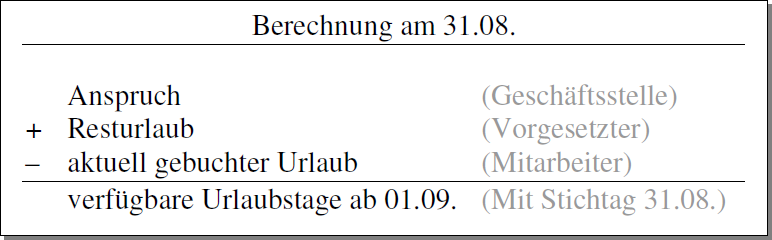
\includegraphics[width=0.70\textwidth]{CIS_Urlaubstool_Berechnung.png}
	\caption{Calculation of Accrued Vacation}
\end{figure}

\section{How to Use the Tool}

The vacation tool is accessed via the CIS page and serves as an extension to the user interface previously used for entering unavailable times. You can still enter and edit unavailable times here just as you did before.
We recommend using the following browsers: Mozilla Firefox or SeaMonkey.

\subsection{Booking a Vacation}

You can view your current accrued vacation and its calculation in the overview at the top left hand of the screen (see Fig. \ref{CIS_urlaubstool_eintragungen}). Clicking the help button will open a detailed description of the calculation.

\begin{figure}
	\centering
	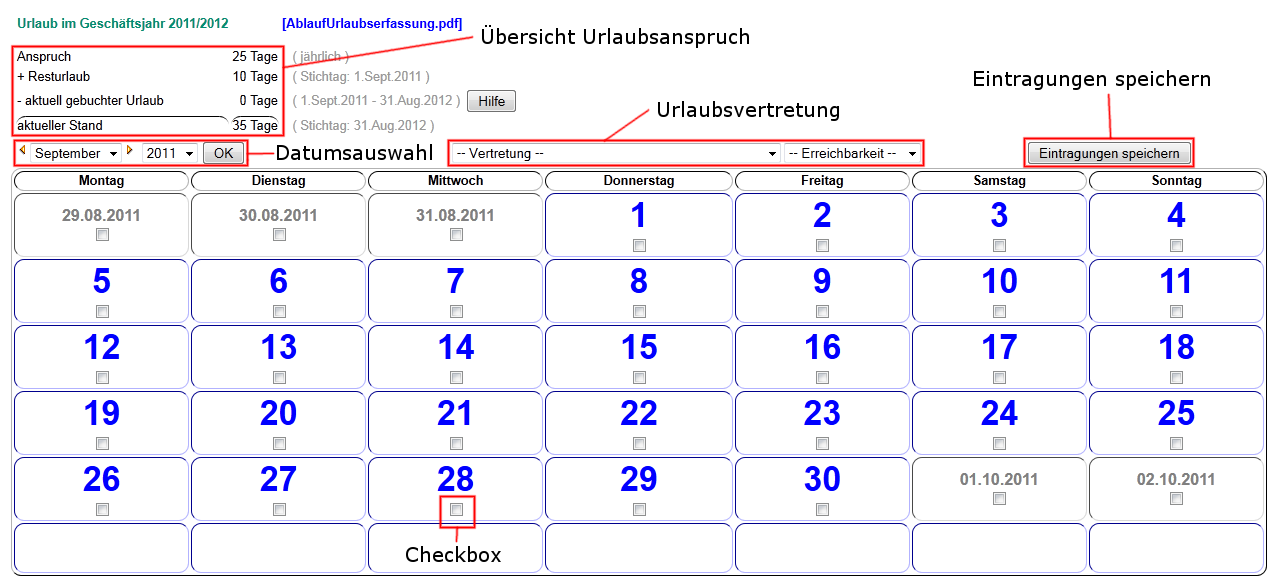
\includegraphics[width=1\textwidth]{CIS_Urlaubstool_Eintragungen.png}
	\caption{Save Vacation}
	\label{CIS_urlaubstool_eintragungen}
\end{figure}

Now select the month and year in which you want to book your vacation. You can select the year and month directly from the drop-down menus and \textbf{by pressing the OK button}, or by scrolling through the calendar with the yellow arrows.

You will see checkboxes underneath each weekday that can be selected or deselected with a simple click of your mouse.  Use these checkboxes to select the days you want to have free for your vacation.

\achtung{National holidays are not currently displayed in the calendar! Please check to ensure there are no national holidays during the time you have selected for your vacation.}

Now use the drop down menus to select your substitute and to indicate how you can be reached during your vacation. 
If you leave your contact information blank, your status will automatically be saved as "'Can not be reached!"'. Now press \textbf{Save Vacation}. 

The vacation time you have booked will now be highlighted in the calendar in light green. At the same time, an email will be sent to your manager with your vacation request and this is also confirmed by a red info text displayed below the calendar.

\info{If there is no manager assigned in the database, this will also be indicated in the info text. Should this be the case, please contact Human Resources.}

If you hold the mouse over a booked vacation (over the number), an infotip will appear with the substitute and information on how you can be reached.

\begin{figure}
	\centering
	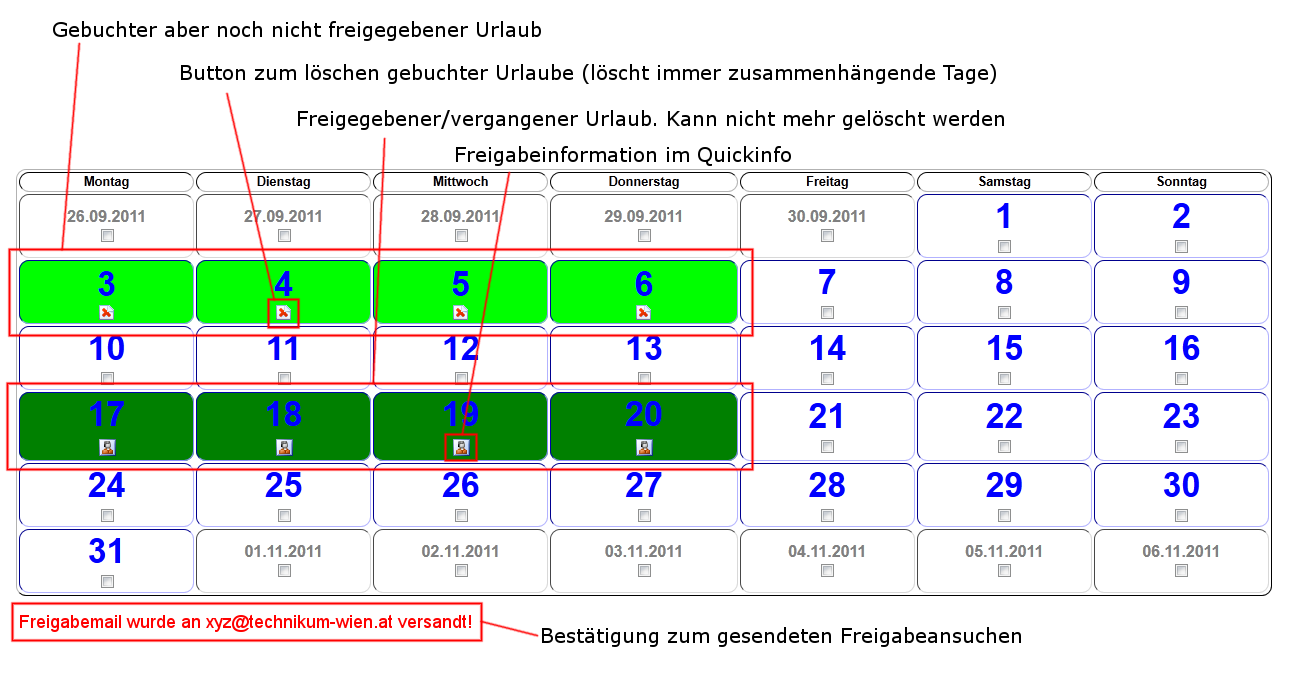
\includegraphics[width=1\textwidth]{CIS_Urlaubstool_Buchungen.png}
	\caption{Booked Vacation }
	\label{CIS_urlaubstool_buchungen}
\end{figure}

\section{Deleting a Booked Vacation}

You can delete a vacation that has been booked but not yet approved by clicking on the x below each vacation day.
Consecutive days are saved as one vacation period and the entire period is deleted again when the delete button is clicked. A click on the delete button in Fig. \ref{CIS_urlaubstool_buchungen}, would therefore delete the entire vacation for August 3rd to the 6th.

{\textit{Please think carefully about your vacation before you book so as not to flood your manager with approval emails and to help avoid any unnecessary confusion.}

\section{Approved Vacation}

After your manager has approved your vacation, it will appear in the vacation tool in dark green and you will no longer be able to delete it.
The delete icon will now be replaced by an information icon. Holding your mouse over this icon will display the infotip where you can see information about who approved your vacation and when.

\achtung{If you book a vacation retroactively for a date in the past (before today's date), it will automatically be marked as approved and you will no longer be able to delete it.}